\documentclass[a4paper,12pt]{report}
\usepackage{graphicx} 		% images
\usepackage[utf8]{inputenc}	% encoding: UTF-8
\usepackage[italian]{babel}	% language
\usepackage[margin=0.5in, includefoot]{geometry}	% margin
\usepackage{scrextend}		% KOMA scripts?
\usepackage{array}			% table width
\usepackage[table]{xcolor}	% table colors
\usepackage{tocloft}			% table of contents
\usepackage{hyperref}			% hyperlinks inside document
\usepackage[italian]{cleveref}	% ^
\usepackage[section]{placeins}
\usepackage{float}
\usepackage{minted}
\usepackage{listings}
\usepackage{color}

\renewcommand{\cftsecleader}{\cftdotfill{\cftdotsep}}
% this command makes a chapter without number and adds it to the toc
\newcommand\chap[1]{
    \chapter*{#1}
    \addcontentsline{toc}{chapter}{#1}
    \markboth{#1}{#1}}

% same as above, but for sections
\newcommand\sect[1]{
    \section*{#1}
    \addcontentsline{toc}{section}{#1}
    \markboth{#1}{#1}}

% colors used in tables and code listings
\definecolor{keywordcolor}{HTML}{2e5abd}
\definecolor{morekwcolor}{HTML}{ff1a8d}
\definecolor{strcolor}{rgb}{0.58,0,0.82}
\definecolor{tablinecolor}{HTML}{999da1}
\definecolor{rowc}{HTML}{abc3f5}

\newcolumntype{P}[1]{>{\centering\arraybackslash}p{#1}}
\renewcommand{\arraystretch}{1.8}
\arrayrulecolor{tablinecolor} % table lines color

\renewcommand\lstlistingname{Quelltext} % change language of section name
% general setup for listings
\lstset{
    language=SQL,
    basicstyle=\ttfamily\footnotesize,
	breakatwhitespace=false,
	breaklines=true,
    tabsize=4,
    columns=fixed,
    showstringspaces=false,
    commentstyle=\color{keywordcolor},
    keywordstyle=\color{blue},
    numberstyle=\color{strcolor},
    stringstyle=\color{strcolor},
    classoffset=3,
    morekeywords={now, datediff},
    keywordstyle=\color{morekwcolor}
}

\title{
\Huge \textbf{Elaborato per il corso di Basi di Dati} \\
[4mm]
\large A.A. 2020/2021 \\
\large Progetto di una base di dati per la gestione di un servizio online
}
\author{Christian Ricci \\
christian.ricci3@studio.unibo.it \\
0000915693}

\begin{document}

\maketitle
\tableofcontents

\chap{Analisi dei requisiti}

Si vuole realizzare un database per gestire un servizio online di videogiochi. Il database dovrà immagazzinare dati relativi ai videogiochi, agli utenti, alle iscrizioni. Gli utenti potranno {giocare} accedendo al servizio e potranno partecipare in sessioni multiplayer. I direttori del servizio potranno aggiungere nuovi videogiochi, consultare statistiche riguardanti gli utenti, etc.

\sect{Definizione delle specifiche in linguaggio naturale}

Il testo ottenuto dall'intervista con l'azienda è il seguente:\\\\

\begin{addmargin}[4em]{4em}
La casa produttrice di videogiochi GameSoft vuole realizzare un servizio online per tutti i videogiochi che ha pubblicato in passato. Gli utenti che si registreranno a questo nuovo servizio potranno accedere ad un catalogo di videogiochi e potranno giocare liberamente a qualunque gioco nel catalogo senza ulteriori costi. Degli utenti si vuole tener traccia del nome utente, della password, dell'email, dell'età e anche di un numero di telefono. Il numero di telefono è opzionale e un utente lo può dare anche dopo essersi registrato.

Al momento della registrazione l'utente potrà scegliere tra tre piani: il primo prevede un periodo gratuito di un mese, che non si potrà rinnovare; a quel punto l'utente deve decidere tra gli altri due piani. Il secondo piano prevede un costo e comporta l'iscrizione al servizio per un mese. Il terzo piano, invece, comporta l'iscrizione per un anno. Si vuole anche memorizzare lo storico delle iscrizioni per ogni utente.

Per ogni videogioco si vuole memorizzare il titolo, il genere, l'anno di rilascio, l'azienda sviluppatrice e il produttore esecutivo. Per ogni utente del servizio si vuole anche dare la possibilità di acquistare una copia fisica di qualunque videogioco, che, però, potrebbe anche non essere disponibile. Ogni videogioco può avere più copie fisiche, ma il prezzo di ogni copia del videogioco è la stessa. Si vuole anche memorizzare lo storico degli acquisti per ogni utente.

Ogni utente inoltre dovrebbe essere in grado di visualizzare il profilo di altri utenti, e di sapere alcune statistiche su quell'utente: le ore di gioco, sia giornaliere che totali; una lista dei giochi più giocati dall'utente; una lista dei giochi preferiti dall'utente. Altre statistiche appaiono per i videogiochi: una lista dei videogiochi più giocati da ogni utente e una lista dei giochi più amati.

Infine, si vuole anche immagazzinare anche alcune informazioni relative al multiplayer. Gli utenti del servizio possono iniziare una sessione di gioco con altri utenti e scegliere un videogioco da giocare: si vuole memorizzare i dati di ogni sessione, che includeranno gli utenti partecipanti, il videogioco scelto e il tempo trascorso a giocare in multiplayer. Si vuole anche mantenere uno storico delle sessioni per ogni utente. Ovviamente, si dovrebbe tener conto che il gioco scelto sia effettivamente un gioco multiplayer. \\\\

\end{addmargin}

\sect{Estrazione dei concetti fondamentali}

I concetti principali sono riassunti in questa tabella.

\begin{table}[h!]
\begin{center}
	\begin{tabular}{ | m{4cm} m{8cm} m{5cm} | }
	\rowcolor{rowc}
	\textbf{Termine} & \textbf{Breve descrizione} & \textbf{Eventuali sinonimi} \\
	Utente & Colui che accede al servizio. Può sottoscrivere nuovi piani, iniziare nuove partite con i videogiochi presenti, creare o partecipare a sezioni, comprare copie fisiche di un gioco. & Account, Profilo \\ \hline
	Videogioco & Indica un videogioco del catalogo. & Titolo \\ \hline
	Copia Videogioco & Indica una copia fisica di un videogioco. Ogni videogioco può avere più copie fisiche. & Copia \\ \hline
	Statistiche & Le statistiche riguardanti un utente e un videogioco. Ce ne sono due principali: le ore di gioco e la preferenza. & \\ \hline
	Piano & Ogni utente deve sottoscrivere un piano per accedere al servizio. & Abbonamento, Iscrizione\\ \hline
	Sessione di gioco & Una partita di un videogioco multiplayer, creata inizialmente da un utente. & Sessione \\ \hline
	\end{tabular}
\end{center}
\caption{La tabella dei concetti principali.}
\end{table}

A seguito della lettura e comprensione dei requisiti richiesti dal cliente, si procede sviluppando un testo che
ne riassuma tutti i concetti e in particolare ne estragga quelli principali, risultando essere in questo modo
meglio fruibile per la realizzazione della base di dati.\\\\

\begin{addmargin}[4em]{4em}
Per ogni \textbf{\textit{utente}} si memorizza nome, cognome, password, email, età e opzionalmente numero di telefono. Ogni utente deve avere un codice univoco, fornito al momento della registrazione.

Un utente può stipulare più \textbf{\textit{piani}}: un piano gratuito è attivato al momento della registrazione. Per ogni tipo di piano c'è una durata e un prezzo e ogni piano viene mantenuto in uno storico, in cui si memorizza anche la data d'inizio (non c'è bisogno della data di scadenza, dato che si può evincere dal tipo di piano). Ogni utente può avere un solo piano attivo alla volta.

Per ogni \textbf{\textit{videogioco}} si deve memorizzare titolo, genere, anno di rilascio, azienda sviluppatrice e produttore esecutivo. Si devono anche memorizzare prezzo e quantità di copie per ogni videogioco. Per ogni copia, invece, si deve memorizzare la data di acquisto.

% Occorre memorizzare in qualche modo le ore di gioco di un utente.

Infine, per ogni \textbf{\textit{sessione}} occorre memorizzare gli utenti partecipanti e il gioco scelto. Dato che non tutti i giochi permettono di giocare in multiplayer, bisogna fare una distinzione tra \textbf{\textit{gioco single player}} e \textbf{\textit{gioco multiplayer}}. Si suppone, inoltre, che un videogioco multiplayer abbia un numero minimo e massimo di giocatori. \\\\

\end{addmargin}

Da questo testo si può anche evincere le principali azioni richieste:

\begin{itemize}
\item Sottoscrivere un nuovo piano per un utente;
\item Visualizzare i piani creati da un utente;
\item Registrare la cancellazione di un piano da parte di un utente;
\item Visualizzare i giochi disponibili nel catalogo;
\item Visualizzare il numero di copie fisiche disponibili di un videogioco;
\item Registrare l'acquisto di una copia di un videogioco;
\item Visualizzare il numero di ore di gioco giornaliero e totale di un utente;
\item Visualizzare i giochi preferiti di un utente;
\item Visualizzare i giochi più giocati e quelli più preferiti;
\item Registrare la creazione di una nuova sessione di gioco;
\item Visualizzare quante sessioni un utente ha creato o ha partecipato per un videogioco;
\end{itemize}


%%%%%%%%%%%%%%%%%%%%%%%%%%%%%%%%%%%%%%%%%%%%
% schema concettuale
%%%%%%%%%%%%%%%%%%%%%%%%%%%%%%%%%%%%%%%%%%%%


\chap{Progetto dello schema concettuale}

La strategia adottata per creare lo schema concettuale è una strategia mista, orientata al bottom-up. Il database è composto da più ambiti, che verranno analizzati e raffinati uno ad uno, per poi creare uno schema finale che comprenda tutto il database.

\sect{Schema scheletro}

L'associazione tra \textbf{Utente} e \textbf{Piano} è abbastanza evidente: un utente può sottoscrivere più piani, ed ogni piano può avere una diversa tipologia. Inoltre, un piano può essere cancellato in qualunque momento dall'utente: per rappresentare questa relazione, si è pensato di creare una gerarchia di tipo \textit{Subset}: \textbf{Piano Cancellato} specializza Piano. L'entità Piano servirà inoltre per rappresentare lo storico dei piani, dato che l'intervista non ha posto particolari requisiti sullo storico. Ogni piano memorizza anche la data e l'ora di acquisto: avere anche l'ora preverrà il problema che un utente non riesca a sottoscrivere un nuovo piano nello stesso giorno (si pensi al caso in cui un utente sottoscriva un piano, poi lo cancelli e ne sottoscriva un altro nello stesso giorno).

L'entità Piano non memorizza alcuna data finale. Per capire il vero stato del piano (in corso, finito o cancellato) e la fine, occorrerà guardare anche la sua tipologia. Dato che ci sono tre diverse tipologie, ognuna con diverse proprietà, si è pensato di reificare la tipologia nell'entità \textbf{Tipologia piano}. Per rappresentare i tre tipi di piano, si è scelto di usare specializzazioni per la più generica Tipologia piano. Riguardo agli identificatori, sia Utente che Piano hanno identificatori univoci, mentre la tipologia piano sarà identificata dal piano in sé.

Un'utente non può stipulare un piano se ha già un piano in corso: questo vincolo non si può esprimere con facilità nello schema concettuale, perciò sarà inserito come \textit{business rule}.

\begin{figure}[!htb]
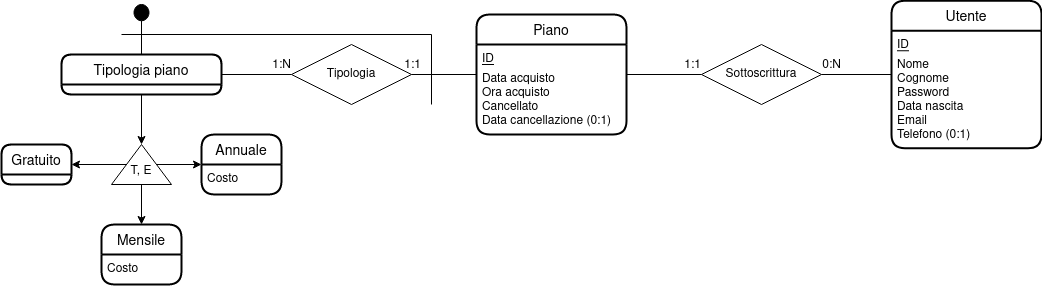
\includegraphics[width=\textwidth]{piano.png}
\caption{Lo schema Entity-Relationship relativo at utenti e piani.}
\label{img:schema_piano}
\end{figure}

Riguardo alle relazioni tra Utente e Videogioco, abbiamo una relazione che riguarda le statistiche dell'utente ed una che riguarda l'acquisto di copie fisiche di un videogioco da parte degli utenti.

Le statistiche di cui si vuole tener traccia sono principalmente due: le ore di gioco dell'utente e i giochi preferiti dell'utente. Per le ore di gioco, si è deciso di rappresentarle tramite un'entità partita: ogni partita di un utente deve essere comunque tracciata per sapere le ore di gioco, quindi ogni partita è rappresentata dall'ID dell'utente, dall'ID del videogioco e dalla data e l'ora di quando è stata iniziata.

Per i giochi preferiti dell'utente, basta avere un'associazione tra Utente e Videogioco che indica la preferenza di un utente per quel videogioco. Mediante operazioni a lato software si potranno estrapolare le altre statistiche richieste, ad esempio la lista dei giochi preferiti e la lista dei giochi più giocati.

Dato che per un videogioco ci possono essere più copie fisiche, si è scelto di creare un entità anche per Copia Videogioco. Il prezzo di ogni copia non riguarda le singole copie, bensì riguarda il gioco in sé, e si suppone inoltre che questo dato rimanga costante nel tempo, per cui è stato messo come attributo di videogioco. Una copia può anche rimanere invenduta, quindi si è pensato di immagazzinare il dato relativo alla data di acquisto come attributo dell'associazione Acquisto. Ogni copia è identificata tramite un codice univoco e l'associazione al videogioco di cui è copia.

\begin{figure}[!htb]
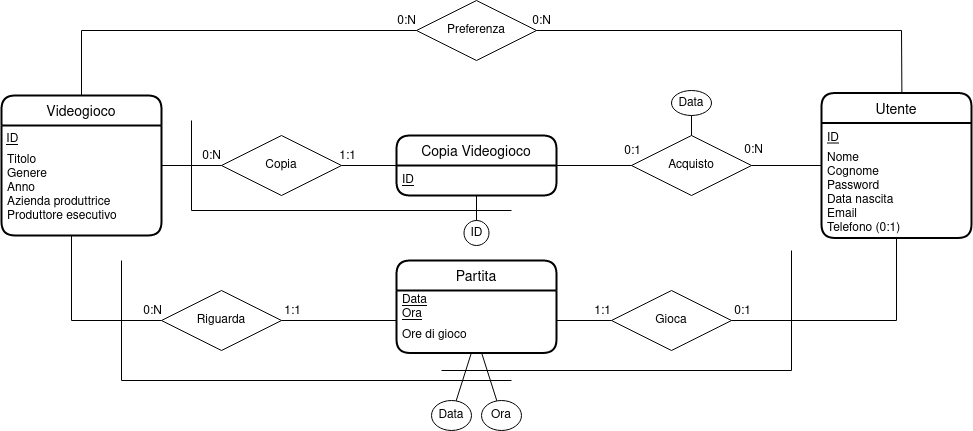
\includegraphics[width=\textwidth]{vg.png}
\caption{Lo schema Entity-Relationship relativo agli utenti, videogiochi, copie e statistiche.}
\label{img:schema_vg}
\end{figure}

L'ambito relativo alle sessioni di gioco multiplayer è il più semplice.

Un \textbf{Videogioco multiplayer} è una specializzazione di Videogioco ed aggiunge gli attributi di numero minimo e massimo di giocatori. Le due entità Utente e Videogioco Multiplayer sono associate all'entità \textbf{Sessione}, che raccoglie dati relativi alla specifica sessione. Una sessione è identificata dall'attributo ID di Sessione e dall'associazione con Videogioco Multiplayer.

Per sottolineare il fatto che un solo utente può dare inizio ad una sessione, mentre più utenti possono parteciparvi, si è optato per due associazioni, \textbf{Creazione} e \textbf{Partecipazione}, tra Utente e Sessione. Rimane un vincolo inespresso: in una sessione, il numero minimo e massimo di giocatori dipende dal videogioco, cosa difficile da esprimere usando il modello ER.

\begin{figure}[H]
\centering{}
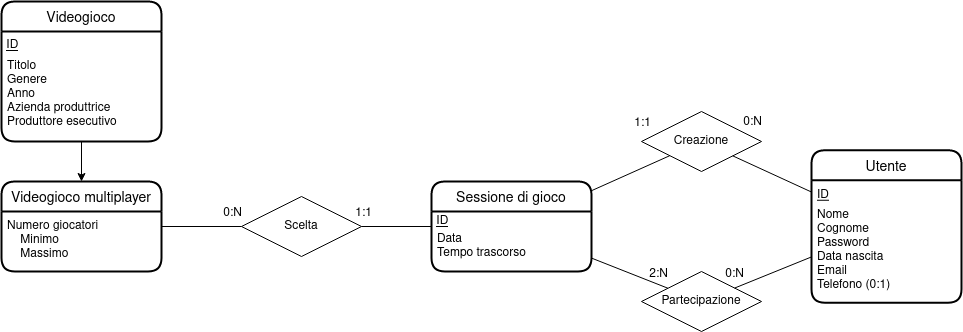
\includegraphics[width=\textwidth]{session.png}
\caption{Lo schema Entity-Relationship relativo alle sessioni.}
\label{img:schema_sessione}
\end{figure}

\newpage

\sect{Schema finale}

\begin{figure}[!htb]
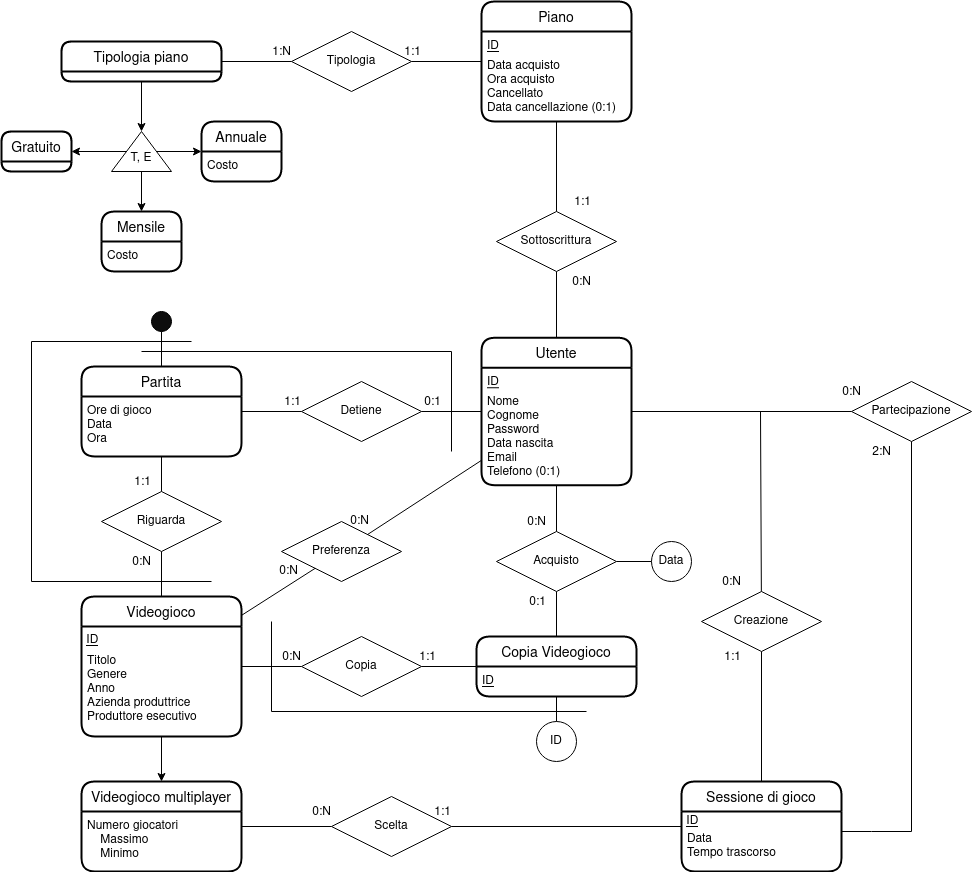
\includegraphics[width=\textwidth]{er_full.png}
\caption{Lo schema Entity-Relationship finale.}
\label{img:schema_finale}
\end{figure}

\newpage


%%%%%%%%%%%%%%%%%%%%%%%%%%%%%%%%%%%%%%%%%%%%
% progettazione logica
%%%%%%%%%%%%%%%%%%%%%%%%%%%%%%%%%%%%%%%%%%%%


\chap{Progettazione logica}

\sect{Stima del volume dei dati}

\begin{table}[h!]
\begin{center}
	\begin{tabular}{ | m{5cm} P{5cm} P{5cm} | }
	\rowcolor{rowc}
	\hline
    \textbf{Concetto} & \textbf{Costrutto} & \textbf{Volume} \\
	Utente & E & 10.000 \\ \hline
	Piano & E & 30.000 \\ \hline
	Sottoscrittura & R & 30.000 \\ \hline
	Tipologia piano & E & 3 \\ \hline
	Piano Cancellato & E & 3000 \\ \hline
	Videogioco & E & 1000 \\ \hline
	Copia Videogioco & E & 10.000 \\ \hline
	Copia & R & 10.000 \\ \hline
	Acquisto & R & 5000 \\ \hline
	Partita & E & 300.000 \\ \hline
	Gioca & R & 300.000 \\ \hline
	Riguarda & R & 300.000 \\ \hline
	Preferenza & R & 7000 \\ \hline
	Videogioco Multiplayer & E & 600 \\ \hline
	Sessione di gioco & E & 100.000 \\ \hline
	Scelta & R & 100.000 \\ \hline
	Creazione & R & 100.000 \\ \hline
	Partecipazione & R & 500.000 \\ \hline
	\end{tabular}
\end{center}
\caption{La tabella dei volumi.}
\end{table}

\sect{Descrizione delle operazioni principali e stima della loro frequenza}

Le operazioni principali sono elencate nella fase di analisi. Segue una tabella delle stime della frequenza per ogni operazione:

\begin{table}[h!]
\begin{center}
	\begin{tabular}{ | P{2cm} m{10cm} m{4cm} | }
	\rowcolor{rowc}
	\hline
	\textbf{Codice} & \textbf{Operazione} & \textbf{Frequenza} \\
	1 & Sottoscrivere un nuovo piano per un utente & 10 al mese \\ \hline
	1 & Visualizzare i piani creati da un utente & 100 al mese \\ \hline
	1 & Registrare la cancellazione di un piano da parte di un utente & 5 al mese \\ \hline
	1 & Visualizzare i giochi disponibili nel catalogo & 1000 al giorno \\ \hline
	1 & Visualizzare il numero di copie fisiche disponibili di un videogioco & 100 al giorno \\ \hline
	1 & Registrare l'acquisto di una copia di un videogioco & 100 al giorno \\ \hline
	1 & Visualizzare il numero di ore di gioco giornaliero e totale di un utente & 5000 al giorno \\ \hline
	1 & Visualizzare i giochi preferiti di un utente & 5000 al giorno \\ \hline
	1 & Visualizzare i giochi più giocati e quelli più preferiti & 5000 al giorno \\ \hline
	1 & Registrare la creazione di una nuova sessione di gioco & 50 al giorno \\ \hline
	1 & Visualizzare quante sessioni un utente ha creato o ha partecipato per un videogioco & 500 al giorno \\ \hline
	\end{tabular}
\end{center}
\caption{Tabella delle stime delle frequenze.}
\end{table}

\newpage

\sect{Schemi di navigazione e tabelle degli accessi}

\subsection*{Login e ricerca di un utente}

\begin{table}[!htb]
\begin{center}
	\begin{tabular}{ | m{5cm} P{4cm} P{4cm} P{4cm} | }
	\rowcolor{rowc}
	\textbf{Concetto} & \textbf{Costrutto} & \textbf{Accessi} & \textbf{Tipo} \\
	Utente         & E & 1 & L \\ \hline
	\rowcolor{rowc}
	\textbf{Totale}: 1L - 9000 al giorno & & & \\
	\hline
	\end{tabular}
\end{center}
\end{table}

\subsection*{Sottoscrivere un nuovo piano per un utente}

Per aggiungere un nuovo piano per l'utente, controllare se questi non abbia già un piano in corso (leggendo da Piano e Tipologia piano), poi scriverlo.

\begin{table}[!htb]
\begin{center}
	\begin{tabular}{ | m{5cm} P{4cm} P{4cm} P{4cm} | }
	\rowcolor{rowc}
	\textbf{Concetto} & \textbf{Costrutto} & \textbf{Accessi} & \textbf{Tipo} \\
	Utente         & E & 1 & L \\ \hline
	Sottoscrittura & R & 1 & L \\ \hline
	Piano          & E & 1 & L \\ \hline
	Tipologia      & R & 1 & L \\ \hline
	Sottoscrittura & R & 1 & S \\ \hline
	Piano          & E & 1 & S \\ \hline
	\rowcolor{rowc}
	\textbf{Totale}: 2L + 1S - 10 al mese & & & \\
	\hline
	\end{tabular}
\end{center}
\end{table}

\subsection*{Visualizzare i piani creati e cancellati da un utente}

Per questa operazione basta prelevare l'ID dell'utente e andare a controllare i piani creati.

\begin{table}[!htb]
\begin{center}
	\begin{tabular}{ | m{5cm} P{4cm} P{4cm} P{4cm} | }
	\rowcolor{rowc}
	\textbf{Concetto} & \textbf{Costrutto} & \textbf{Accessi} & \textbf{Tipo} \\
	Utente         & E & 1 & L \\ \hline
	Sottoscrittura & E & 1 & L \\ \hline
	Piano 		 & E & 1 & L \\ \hline
	\rowcolor{rowc}
	\textbf{Totale}: 2 L - 100 al mese & & & \\
	\hline
	\end{tabular}
\end{center}
\end{table}

\newpage

\subsection*{Registrare la cancellazione di un piano da parte di un utente}

Prima bisogna guardare il piano in corso di un utente, poi si registra la cancellazione.

\begin{table}[!htb]
\begin{center}
	\begin{tabular}{ | m{5cm} P{4cm} P{4cm} P{4cm} | }
	\rowcolor{rowc}
	\textbf{Concetto} & \textbf{Costrutto} & \textbf{Accessi} & \textbf{Tipo} \\
	Utente           & E & 1 & L \\ \hline
	Piano    		   & E & 1 & L \\ \hline
	Tipologia		   & R & 1 & L \\ \hline
	Tipologia piano  & E & 1 & L \\ \hline
	Sottoscrittura   & R & 1 & L \\ \hline
	Piano Cancellato & E & 1 & S \\ \hline
	\rowcolor{rowc}
	\textbf{Totale}: 2L + 1S - 5 al mese & & & \\
	\hline
	\end{tabular}
\end{center}
\end{table}

\subsection*{Visualizzare i giochi disponibili nel catalogo}

Un utente, per poter visualizzare il catalogo, deve avere almeno un piano in corso.

\begin{table}[h!]
\begin{center}
	\begin{tabular}{ | m{4cm} P{4cm} P{4cm} P{4cm} | }
	\rowcolor{rowc}
	\textbf{Concetto} & \textbf{Costrutto} & \textbf{Accessi} & \textbf{Tipo} \\
	Utente 		   & E & 1 & L \\ \hline
	Sottoscrittura   & R & 1 & L \\ \hline
	Piano 		   & E & 1 & L \\ \hline
	Tipologia		   & R & 1 & L \\ \hline
	Tipologia piano  & E & 1 & L \\ \hline
	Videogioco       & E & 1 & L \\ \hline
	\rowcolor{rowc}
	\textbf{Totale}: 1L - 1000 al giorno & & & \\
	\hline
	\end{tabular}
\end{center}
\end{table}

\subsection*{Visualizzare il numero di copie fisiche disponibili di un videogioco}

L'input è il nome di un videogioco. Per vedere se una copia è disponibile, bisogna guardare anche gli acquisti.

\begin{table}[h!]
\begin{center}
	\begin{tabular}{ | m{4cm} P{4cm} P{4cm} P{4cm} | }
	\rowcolor{rowc}
	\textbf{Concetto} & \textbf{Costrutto} & \textbf{Accessi} & \textbf{Tipo} \\
	Videogioco       & E & 1 & L \\ \hline
	Copia		   & R & 1 & L \\ \hline
	Copia Videogioco & E & 1 & L \\ \hline
	Acquisto 		   & R & 1 & L \\ \hline
	\rowcolor{rowc}
	\textbf{Totale}: 2L - 100 al giorno & & & \\
	\hline
	\end{tabular}
\end{center}
\end{table}

\newpage

\subsection*{Registrare l'acquisto di una copia di un videogioco}

Basta aggiungere un nuovo acquisto.

\begin{table}[h!]
\begin{center}
	\begin{tabular}{ | m{4cm} P{4cm} P{4cm} P{4cm} | }
	\rowcolor{rowc}
	\textbf{Concetto} & \textbf{Costrutto} & \textbf{Accessi} & \textbf{Tipo} \\
	Acquisto & R & 1 & S \\ \hline
	\rowcolor{rowc}
	\textbf{Totale}: 1L + 1S - 100 al giorno & & & \\
	\hline
	\end{tabular}
\end{center}
\end{table}

\subsection*{Visualizzare il numero di ore di gioco giornaliero e totale di un utente}

Basta guardare solo partita.

\begin{table}[h!]
\begin{center}
	\begin{tabular}{ | m{4cm} P{4cm} P{4cm} P{4cm} | }
	\rowcolor{rowc}
	\textbf{Concetto} & \textbf{Costrutto} & \textbf{Accessi} & \textbf{Tipo} \\
	Utente  & E & 1 & L \\ \hline
	Gioca   & R & 2 & L \\ \hline
	Partita & E & 2 & L \\ \hline
	\rowcolor{rowc}
	\textbf{Totale}: 4L - 5000 al giorno & & & \\
	\hline
	\end{tabular}
\end{center}
\end{table}

\newpage

\subsection*{Visualizzare i giochi preferiti di un utente}

\begin{table}[h!]
\begin{center}
	\begin{tabular}{ | m{4cm} P{4cm} P{4cm} P{4cm} | }
	\rowcolor{rowc}
	\textbf{Concetto} & \textbf{Costrutto} & \textbf{Accessi} & \textbf{Tipo} \\
	Utente     & E & 1 & L \\ \hline
	Preferenza & R & 1 & L \\ \hline
	Videogioco & E & 1 & L \\ \hline
	\rowcolor{rowc}
	\textbf{Totale}: 3L - 5000 al giorno & & & \\
	\hline
	\end{tabular}
\end{center}
\end{table}

\subsection*{Visualizzare i giochi più giocati e quelli più preferiti}

Per visualizzare quelli più giocati, occorre guardare Partita. Per visualizzare quelli preferiti, occorre guardare Preferenza.

\begin{table}[h!]
\begin{center}
	\begin{tabular}{ | m{4cm} P{4cm} P{4cm} P{4cm} | }
	\rowcolor{rowc}
	\textbf{Concetto} & \textbf{Costrutto} & \textbf{Accessi} & \textbf{Tipo} \\
	Videogioco & E & 1 & L \\ \hline
	Riguarda	  & R & 1 & L \\ \hline
	Partita    & E & 1 & L \\ \hline
	Preferenza & R & 1 & L \\ \hline
	\rowcolor{rowc}
	\textbf{Totale}: 4L - 5000 al giorno & & & \\
	\hline
	\end{tabular}
\end{center}
\end{table}

\newpage

\subsection*{Registrare la creazione di una nuova sessione di gioco}

Questo comporta avere l'utente creatore, gli utenti partecipanti e il videogioco scelto e comporta anche aggiornare la creazione e la partecipazione da parte di un utente. Si suppone che in media avremo 5 partecipanti.
Prima di registrare bisogna vedere il numero massimo e minimo di utenti.
Questa query registra solo l'inizio di una sessione, quindi il tempo trascorso bisognerà metterlo in un secondo momento.

\begin{table}[h!]
\begin{center}
	\begin{tabular}{ | m{4cm} P{4cm} P{4cm} P{4cm} | }
	\rowcolor{rowc}
	\textbf{Concetto} & \textbf{Costrutto} & \textbf{Accessi} & \textbf{Tipo} \\
	Sessione		         & E & 1 & S \\ \hline
	Scelta		         & R & 2 & S \\ \hline
	Videogioco multiplayer & E & 2 & L \\ \hline
	Creazione              & R & 1 & S \\ \hline
	Partecipazione         & R & 5 & S \\ \hline
	Utente                 & E & 6 & L \\ \hline
	\rowcolor{rowc}
	\textbf{Totale}: - 50 al giorno & & & \\
	\hline
	\end{tabular}
\end{center}
\end{table}

\subsection*{Visualizzare quante sessioni un utente ha creato o ha partecipato per un videogioco}

\begin{table}[h!]
\begin{center}
	\begin{tabular}{ | m{4cm} P{4cm} P{4cm} P{4cm} | }
	\rowcolor{rowc}
	\textbf{Concetto} & \textbf{Costrutto} & \textbf{Accessi} & \textbf{Tipo} \\
	Utente         & E & 1 & L \\ \hline
	Partecipazione & R & 1 & L \\ \hline
	Creazione      & R & 1 & L \\ \hline
	Sessione       & E & 1 & L \\ \hline
	Scelta		   & R & 1 & L \\ \hline
	Videogioco     & E & 1 & L \\ \hline
	\rowcolor{rowc}
	\textbf{Totale}: 500 al giorno & & & \\
	\hline
	\end{tabular}
\end{center}
\end{table}

\subsection*{Profitto mensile del servizio}

\begin{table}[h!]
\begin{center}
	\begin{tabular}{ | m{4cm} P{4cm} P{4cm} P{4cm} | }
	\rowcolor{rowc}
	\textbf{Concetto} & \textbf{Costrutto} & \textbf{Accessi} & \textbf{Tipo} \\
	Piano		& E & 1 & L \\ \hline
	\rowcolor{rowc}
	\textbf{Totale}: 500 al giorno & & & \\
	\hline
	\end{tabular}
\end{center}
\end{table}


%%%%%%%%%%%%%%%%%%%%%%%%%%%%%
% schema logico
%%%%%%%%%%%%%%%%%%%%%%%%%%%%%


\sect{Raffinamento dello schema}

\begin{itemize}

\item \textbf{Eliminazione delle gerarchie} \\
Nello schema concettuale compaiono due gerarchie:
	\begin{itemize}
	\item La gerarchia riguardante la tipologia dei piani, che descrive ogni tipologia esistente;
	\item La gerarchia dei videogiochi multiplayer, che è un semplice sottoinsieme della più generica entità videogioco;
	\item La gerarchia dei piani, anch'essa un semplice sottoinsieme;
	\end{itemize}

Per la gerarchia delle tipologie, si è deciso di fare un collasso verso l'alto: un unica tabella \textbf{Tipologia piano} conterrà le tre tipologie, contenendo inoltre il costo e la durata (per il piano gratuito, si metterà semplicemente un costo uguale a zero).

Per i videogiochi multiplayer, la decisione invece è stata di fare un collasso verso il figlio: si crea una tabella \textbf{Videogioco multiplayer} che avrà un campo ID, chiave esterna alla tabella videogioco.

La stessa decisione che si è presa per i videogiochi multiplayer è stata presa anche per i piani: avremo anche una tabella per \textbf{Piano cancellato}, che avrà una chiave esterna ID Piano, corrispondente al Piano.

\item \textbf{Eliminazione degli attributi composti} \\
L'unico attributo composto presente nello schema è dentro videogioco multiplayer: questo attributo riguarda il numero massimo e minimo di giocatori per il videogioco ed è molto facile scomporlo in due attributi (numero massimo giocatori e numero minimo giocatori).

\item \textbf{Scelta delle chiavi primarie}
Nello schema sono già evidenziate le chiavi primarie per ogni entità principale (Utente, Videogioco, Copia Videogioco, Piano, Sessione); Per le altre entità, le chiavi esterne evidenziate nello schema concettuale possono essere tradotte senza ambiguità in chiavi primarie (ad esempio, l'entità Partita ha come chiave primaria le due chiavi esterne alle tabelle Utente e Videogioco; molte altre entità seguiranno questo stesso pattern).

Una nota particolare riguarda l'entità Tipologia piano: per la tabella corrispondente è stata usata la colonna tipologia come chiave primaria; inoltre è la tabella Piano che referenzia Tipologia piano.

Un'altra nota particolare riguarda l'associazione Preferito, che nella conversione a tabella ha acquisito come chiave primaria la tupla ID Utente - ID Videogioco.

\item \textbf{Eliminazione degli identificatori esterni}

Nel passaggio da schema ER a schema logico, sono state eliminate le seguenti relazioni:

\begin{itemize}
\item Sottoscrittura, importando ID Utente in Piano;
\item Tipologia, importando l'attributo tipologia in Piano;
\item Gioca, importando ID Utente in Partita;
\item Riguarda, importando ID Videogioco in Partita;
\item Acquisto, importando ID Utente in Copia videogioco e aggiungendo un attributo Data acquisto;
\item Copia, importando ID Videogioco in Copia videogioco;
\item Scelta, importando ID Videogioco in Sessione;
\item Creazione, importando ID Utente in Sessione e rinominandolo in ID Utente Creatore;
\end{itemize}

\end{itemize}

\sect{Analisi delle ridondanze}

\sect{Traduzione di entità e associazioni in relazioni}

\begin{itemize}

\item \textbf{Utente}(\underline{ID}, Nome, Cognome, Password, E-Mail, Telefono*)
\item \textbf{Videogioco}(\underline{ID}, Titolo, Genere, Anno, Azienda produttrice, Direttore principale, Prezzo copia fisica)
\item \textbf{Copia videogioco}(\underline{ID}, \underline{ID videogioco}, ID utente*, Data acquisto*) \\
FK: ID utente REFERENCES \textbf{Utente} \\
FK: ID videogioco REFERENCES \textbf{Videogioco}
\item \textbf{Acquisto}(\underline{ID copia}, \underline{ID utente}, Data acquisto) \\
FK: ID utente REFERENCES \textbf{Utente} \\
FK: ID copia REFERENCES \textbf{Copia Videogioco}
\item \textbf{Partita}(\underline{ID utente}, \underline{ID videogioco}, \underline{Data}, \underline{Ora}, Ore di gioco) \\
FK: ID utente REFERENCES \textbf{Utente} \\
FK: ID videogioco REFERENCES \textbf{Videogioco}
\item \textbf{Preferenza}(\underline{ID utente}, \underline{ID videogioco}) \\
FK: ID utente REFERENCES \textbf{Utente} \\
FK: ID videogioco REFERENCES \textbf{Videogioco}
\item \textbf{Videogioco multiplayer}(\underline{ID videogioco}, Numero minimo giocatori, Numero massimo giocatori) \\
FK: ID videogico REFERENCES \textbf{Videogioco}
\item \textbf{Piano}(\underline{ID}, ID utente, Tipologia, Data acquisto, Ora acquisto) \\
FK: Tipologia REFERENCES \textbf{Tipologia piano} \\
FK: ID utente REFERENCES \textbf{Utente}
\item \textbf{Tipologia piano}(\underline{Tipologia}, Costo)
\item \textbf{Piano cancellato}(\underline{ID}, Data cancellazione, Ora cancellazione) \\
FK: ID REFERENCES \textbf{Piano}
\item \textbf{Sessione}(\underline{ID}, ID videogioco, ID creatore, Data, Tempo trascorso) \\
FK: ID videogioco REFERENCES \textbf{Videogioco} \\
FK: ID creatore REFERENCES \textbf{Utente}
\item \textbf{Partecipazione}(\underline{ID utente}, \underline{ID sessione}) \\
FK: ID utente REFERENCES \textbf{Utente} \\
FK: ID sessione REFERENCES \textbf{Sessione}
\end{itemize}

\newpage

\sect{Schema relazionale finale}

\begin{figure}[!htb]
\centering{}
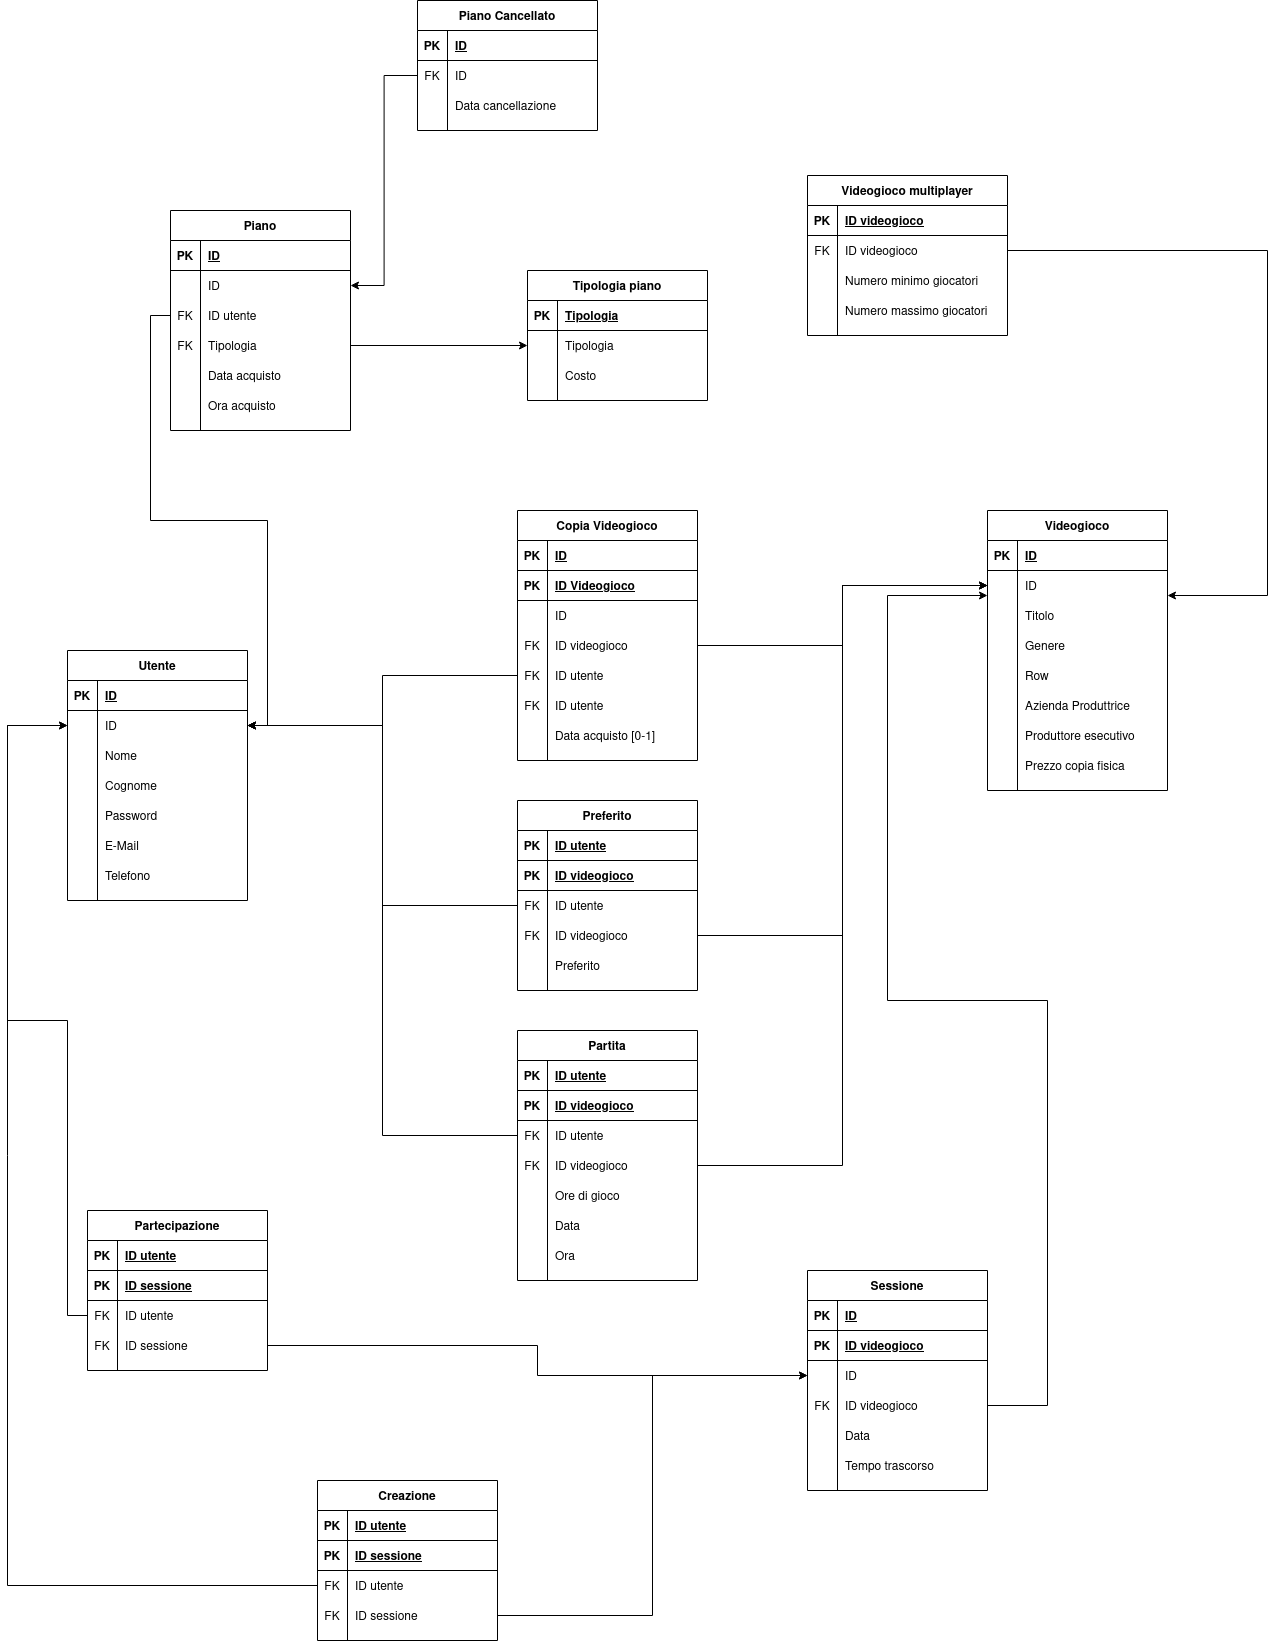
\includegraphics[width=\textwidth]{logical.png}
\caption{Lo schema logico finale.}
\label{img:schema_logico_finale}
\end{figure}

\newpage

\sect{Costruzione delle tabelle in linguaggio SQL}

\usemintedstyle{borland}
\begin{lstlisting}

create table Utente (
    id              int                 primary key auto_increment,
    nome            varchar(255)        not null,
    cognome         varchar(255)        not null,
    password        varchar(255)        not null,
    email           varchar(255)        not null,
    telefono        int
);

create table Videogioco (
    id              int                 primary key auto_increment,
    titolo          varchar(255)        not null,
    genere          varchar(255),
    anno            year,
    azienda         varchar(255),
    produttore      varchar(255),
    prezzo          int
);

create table CopiaVideogioco (
    id              int                 primary key auto_increment,
    id_vg           int                 not null references Videogioco(id)
);

create table Acquisto (
    id_copia        int                 not null references CopiaVideogioco(id),
    id_usr          int                 not null references Utente(id),
    data_acquisto   datetime,
    unique (id_copia, id_usr)
);

create table Partita (
    id_usr          int                 not null references Utente(id),
    id_vg           int                 not null references Videogioco(id),
    data            datetime            not null,
    ore_gioco       int,
    unique (id_usr, id_vg, data)
);

create table Preferenza (
    id_usr          int                 not null references Utente(id),
    id_vg           int                 not null references Videogioco(id),
    unique (id_usr, id_vg)
);

create table VideogiocoMultiplayer (
    id_vg           int                 primary key references Videogioco(id),
    min_giocatori   int                 default 1,
    max_giocatori   int
);

create table TipologiaPiano (
    tipologia       enum('Gratuito',
                         'Mensile',
                         'Annuale')     primary key,
    costo           int                 not null
);

create table Piano (
    id              int                 primary key auto_increment,
    id_usr          int                 not null references Utente(id),
    tipologia       enum('Gratuito',
                         'Mensile',
                         'Annuale')     not null references TipologiaPiano(tipologia),
    data_acquisto   date                not null,
    ora_acquisto    time                not null
);

create table PianoCancellato (
    id              int                 primary key references Piano(id),
    data_canc       date                not null,
    ora_canc        time                not null
);

create table Sessione (
    id              int                 primary key,
    id_vg           int                 not null references VideogiocoMultiplayer(id_vg),
    id_creatore     int                 not null references Utente(id),
    data            date,
    tempo_trascorso int
);

create table Partecipazione (
    id_usr          int                 not null references Utente(id),
    id_session      int                 not null references Sessione(id),
    unique(id_usr, id_session)
);

\end{lstlisting}

\sect{Traduzione delle operazioni in query SQL}

% used when user clicks on 'login as user' button
\subsection*{Login e ricerca di un utente}
\begin{lstlisting}
select *
from Utente u
where u.nome = nome_utente and u.password = password
\end{lstlisting}

% Login e ricerca di un utente                                                          login button, or searching for user
% Sottoscrivere un nuovo piano per un utente                                            create new plan button
% Visualizzare i piani creati e cancellati da un utente admin side                      admin side
% Registrare la cancellazione di un piano da parte di un utente                         delete plan button
% Visualizzare i giochi disponibili nel catalogo                                        obvious
% Visualizzare il numero di copie fisiche disponibili di un videogioco                  when clicking on a videogame
% Registrare l'acquisto di una copia di un videogioco                                   buy copy button
% Visualizzare il numero di ore di gioco giornaliero e totale di un utente              user profile
% Visualizzare i giochi preferiti di un utente                                          user profile
% Visualizzare i giochi più giocati e quelli più preferiti                              user/admin side
% Registrare la creazione di una nuova sessione di gioco                                starting session (?)
% Visualizzare quante sessioni un utente ha creato o ha partecipato per un videogioco   user profile (or get rid of it)
% Profitto mensile del servizio                                                         admin side

\subsection*{Visualizzare i piani creati e cancellati da un utente}

\verb id_utente corrisponde all'ID dell'utente di cui visualizzare i piani. La prima query restituisce i piani creati, la seconda i piani cancellati.

\begin{lstlisting}
select *
from Piano p
where p.id_usr = id_utente;
\end{lstlisting}

\begin{lstlisting}
select *
from Piano p, PianoCancellato pc
where p.id_usr = id_utente
and p.id = pc.id;
\end{lstlisting}

\subsection*{Sottoscrivere un nuovo piano per un utente}

\begin{lstlisting}
select *
from Piano p
where p.id_usr = id_utente
and datediff(now(), p.data_fine) < 0
and p.id not in (select pc.id
                 from PianoCancellato pc);
\end{lstlisting}

Se la query restituisce un risultato vuoto, si può procedere all'inserimento:

\begin{lstlisting}
insert into Piano(id, id_usr, tipologia, data_acquisto, ora_acquisto, data_fine) values(?, ?, ?, ?);
\end{lstlisting}

\subsection*{Registrare la cancellazione di un piano da parte di un utente}

Questa query è simile all'ultima: si cerca l'ID del piano corrente dell'utente, e se esiste, si aggiornano i piani cancellati.

\begin{lstlisting}
select id
if exists in (select p.id
              from Piano p
              where p.id_usr = id_utente
              where datediff(now(), p.data_fine) < 0
              and p.id not in (select pc.id
                               from PianoCancellato pc))

insert into PianoCancellato values (id, now(), now())
\end{lstlisting}

\subsection*{Ricerca di un videogioco nel catalogo}

\begin{lstlisting}
% select titolo, genere, anno, azienda, produttore, prezzo
% from Videogioco
% order by titolo;
\end{lstlisting}

\subsection*{Visualizzare il numero di copie fisiche disponibili di un videogioco}

\begin{lstlisting}
select count(*)
from CopiaVideogioco cv
where cv.id_vg = id_videogioco;
\end{lstlisting}

\subsection*{Registrare l'acquisto di una copia di un videogioco}

La query deve prendere l'ID di una qualsiasi copia che non sia stata acquistata. Per semplicità, prendiamo sempre l'ID minore.

\begin{lstlisting}
select min(cv.id) as id
from CopiaVideogioco cv
where cv.id_vg = id_videogioco
and cv.id not in (select a.id from Acquisto);
\end{lstlisting}

\subsection*{Visualizzare il numero di ore di gioco giornaliero e totale di un utente}

\begin{lstlisting}
select count(p.ore_gioco) as ore_totali
from Partita p
where p.id_usr = id_utente;

select avg(p.ore_gioco) as ore_giornaliere
from Partita p
where p.id_usr = id_utente
group by p.data;
\end{lstlisting}

\subsection*{Visualizzare i giochi preferiti di un utente}

\begin{lstlisting}
select vg.titolo as nome_videogioco
from Videogioco vg, Preferenza p
where vg.id = p.id_vg and u.id = p.id_usr
and u.nome = nome_utente;
\end{lstlisting}

\subsection*{Visualizzare i giochi più giocati e quelli più preferiti}
\subsection*{Registrare la creazione di una nuova sessione di gioco}
\subsection*{Visualizzare quante sessioni un utente ha creato o ha partecipato per un videogioco}
\subsection*{Profitto mensile del servizio}

\chap{Progettazione dell'applicazione}

\sect{Descrizione dell'architettura dell'applicazione}

\end{document}
